\documentclass{article}%
\usepackage[T1]{fontenc}%
\usepackage[utf8]{inputenc}%
\usepackage{lmodern}%
\usepackage{textcomp}%
\usepackage{lastpage}%
\usepackage[head=40pt,margin=0.5in,bottom=0.6in]{geometry}%
\usepackage{graphicx}%
%
\title{\textbf{EE UU amenaza con responder si realizan actos en contra de Guaidó}}%
\author{EFE}%
\date{04/03/2019}%
%
\begin{document}%
\normalsize%
\maketitle%
\textbf{URL: }%
http://www.el{-}nacional.com/noticias/amenaza{-}con{-}responder{-}realizan{-}actos{-}contra{-}guaido\_273303\newline%
%
\textbf{Periodico: }%
EN, %
ID: %
273303, %
Seccion: %
EE UU\newline%
%
\textbf{Palabras Claves: }%
Nicolás Maduro, Estados Unidos\newline%
%
\textbf{Derecho: }%
2.1%
, Otros Derechos: %
\newline%
%
\textbf{\textit{El asesor de Seguridad Nacional de la Casa Blanca sostuvo que su gobierno pretende~crear una coalición amplia internacional para reemplazar a Nicolás Maduro~}}%
\newline%
\newline%
%
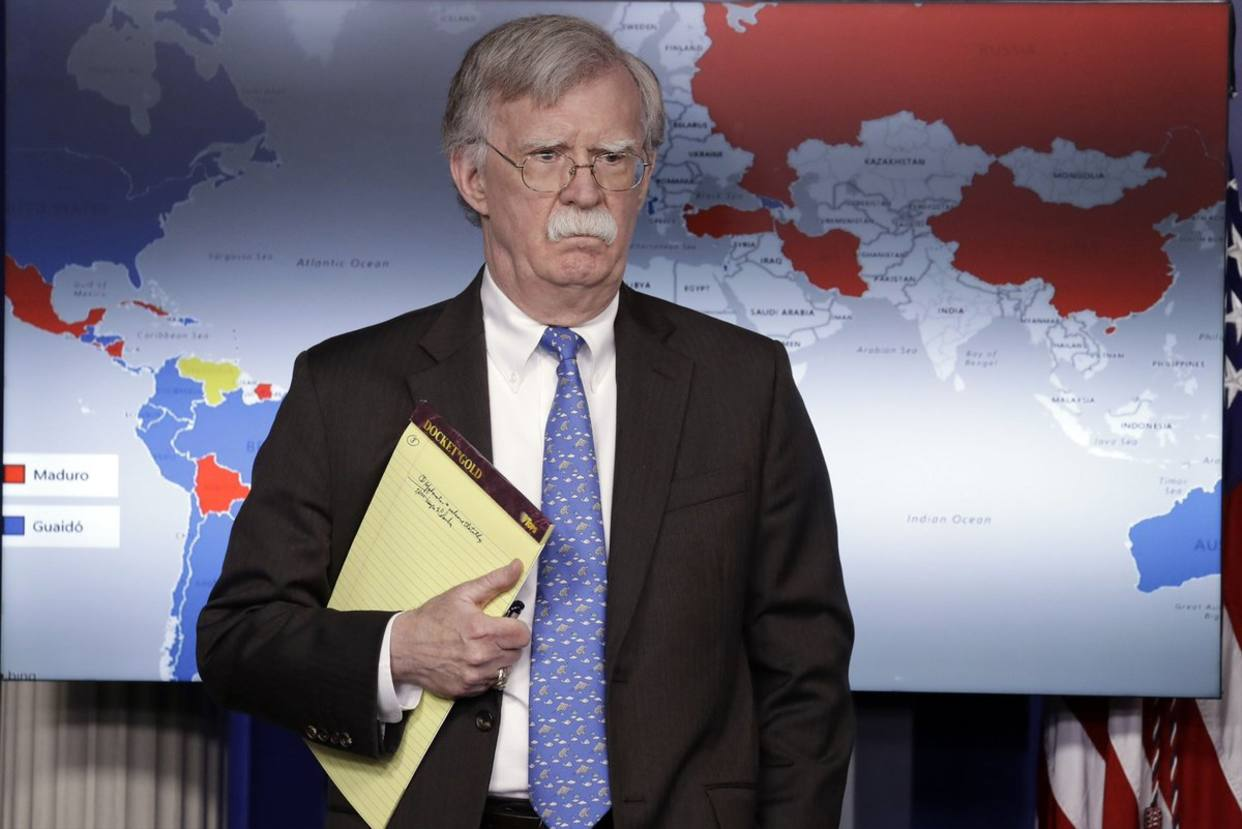
\includegraphics[width=300px]{EN_273303.jpg}%
\newline%
%
El asesor de Seguridad Nacional de la Casa Blanca, John Bolton, advirtió este lunes~que su país lanzará una respuesta fuerte y significante~a cualquier acto~contra~el~regreso a Venezuela~del líder opositor, Juan~Guaidó.%
\newline%
%
"El presidente interino Juan~Guaidó~ha anunciado su planeada vuelta a Venezuela. Cualquier~amenaza~o acto~contra~su retorno~seguro~se encontrará con una respuesta fuerte y significante por parte de Estados Unidos y de la comunidad internacional", advirtió Bolton.%
\newline%
%
Guaidó, que se juramentó presidente interino~del país el pasado 23 de enero, dijo este domingo que si es detenido en su regreso a Caracas sería uno de los últimos errores que cometa~Nicolás Maduro, al que tachó de dictatorial.%
\newline%
%
"Si se atreve el régimen a secuestrarme será uno de los últimos errores, sin duda, que cometa", apuntó~Guaidó, que ha sido reconocido por medio centenar de naciones, en una declaración que transmitió por redes sociales en la que dio detalle de la gira que hizo esta semana por cinco países, Colombia, Brasil, Paraguay, Argentina y Ecuador, en busca de apoyo político.%
\newline%
%
El opositor abandonó el pasado 22 de febrero el territorio venezolano pese a la prohibición de salir del país, por lo~que está investigando su proclamación como presidente interino, lo que el Tribunal Supremo de Justicia no avala ya que solo reconoce a Maduro como jefe de Estado.%
\newline%
%
En una entrevista~a la cadena de televisión CNN, Bolton afirmó que~EE UU~pretende~una "coalición amplia" internacional para reemplazar a Nicolás Maduro~y a todo el régimen corrupto.%
\newline%
%
"Me gustaría ver una coalición tan amplia como podamos reunir para reemplazar a Maduro, reemplazar a su régimen corrupto. Eso es lo que estamos intentando hacer", indicó Bolton.%
\newline%
%
\end{document}